% Created 2024-01-20 sáb 13:21
% Intended LaTeX compiler: pdflatex
\documentclass[a4paper]{article}
\usepackage[utf8]{inputenc}
\usepackage[T1]{fontenc}
\usepackage{graphicx}
\usepackage{longtable}
\usepackage{wrapfig}
\usepackage{rotating}
\usepackage[normalem]{ulem}
\usepackage{amsmath}
\usepackage{amssymb}
\usepackage{capt-of}
\usepackage{hyperref}
\usepackage[spanish]{babel}
\usepackage[usenames,dvipsnames]{color} % Required for custom colors
\renewcommand{\ttdefault}{pcr} % MONOESPACIO CON NEGRIT
\usepackage{lastpage}
\usepackage{listings}
\usepackage{listingsutf8}
\renewcommand{\lstlistingname}{Listado}
\lstset{frame=single,inputencoding=utf8,basicstyle=\scriptsize\ttfamily,showstringspaces=false,numbers=none}
\definecolor{MyDarkGreen}{rgb}{0.0,0.4,0.0} % This is the color used for comments
\lstset{ breaklines=true, postbreak=\mbox{\textcolor{red}{$\hookrightarrow$}\space}, keywordstyle=\bfseries, keywordstyle=[1]\color{Blue}\bfseries,  keywordstyle=[2]\color{Purple}\bfseries,  keywordstyle=[3]\color{Blue}\underbar,   identifierstyle=,   commentstyle=\usefont{T1}{pcr}{m}{sl}\color{MyDarkGreen}\small,   stringstyle=\color{Purple},   showstringspaces=false,   tabsize=2,   morecomment=[l][\color{Blue}]{...} }
\lstset{literate=  {á}{{\'a}}1 {é}{{\'e}}1 {í}{{\'i}}1 {ó}{{\'o}}1 {ú}{{\'u}}1   {Á}{{\'A}}1 {É}{{\'E}}1 {Í}{{\'I}}1 {Ó}{{\'O}}1 {Ú}{{\'U}}1   {à}{{\`a}}1 {è}{{\`e}}1 {ì}{{\`i}}1 {ò}{{\`o}}1 {ù}{{\`u}}1   {À}{{\`A}}1 {È}{{\'E}}1 {Ì}{{\`I}}1 {Ò}{{\`O}}1 {Ù}{{\`U}}1   {ä}{{\"a}}1 {ë}{{\"e}}1 {ï}{{\"i}}1 {ö}{{\"o}}1 {ü}{{\"u}}1   {Ä}{{\"A}}1 {Ë}{{\"E}}1 {Ï}{{\"I}}1 {Ö}{{\"O}}1 {Ü}{{\"U}}1   {â}{{\^a}}1 {ê}{{\^e}}1 {î}{{\^i}}1 {ô}{{\^o}}1 {û}{{\^u}}1   {Â}{{\^A}}1 {Ê}{{\^E}}1 {Î}{{\^I}}1 {Ô}{{\^O}}1 {Û}{{\^U}}1   {œ}{{\oe}}1 {Œ}{{\OE}}1 {æ}{{\ae}}1 {Æ}{{\AE}}1 {ß}{{\ss}}1   {ű}{{\H{u}}}1 {Ű}{{\H{U}}}1 {ő}{{\H{o}}}1 {Ő}{{\H{O}}}1   {ç}{{\c c}}1 {Ç}{{\c C}}1 {ø}{{\o}}1 {å}{{\r a}}1 {Å}{{\r A}}1   {€}{{\euro}}1 {£}{{\pounds}}1 {«}{{\guillemotleft}}1   {»}{{\guillemotright}}1 {ñ}{{\~n}}1 {Ñ}{{\~N}}1 {¿}{{?`}}1 }
\usepackage{caption}
\usepackage{attachfile}
\usepackage[margin=1.5cm,includeheadfoot,includehead,includefoot]{geometry}
\hypersetup{colorlinks,linkcolor=black}
\usepackage{fancyhdr}
\pagestyle{fancyplain}
\chead{}
\lhead{}
\rhead{}
\cfoot{}
\lfoot{\begin{footnotesize}alvaro.gonzalezsotillo@educa.madrid.org\end{footnotesize}}
\rfoot{\begin{footnotesize}\thepage / \pageref{LastPage}\end{footnotesize}}
\usepackage[skins]{tcolorbox}
\usepackage{multicol}
\usepackage{changepage} %ajdustwidth
\usepackage{fancybox}
\usepackage{attachfile2}
\lhead{Extraordinaria 2021 (es el \\lhead)}
\rhead{Administración y Gestión de Bases de Datos (es el \\rhead)}
\lhead{Red IP simple \textit{Packet Tracer}}
\rhead{Planificación y administración de redes}
\usepackage{svg}
\usepackage{letltxmacro}
\LetLtxMacro{\originalincludegraphics}{\includegraphics}
\renewcommand{\includegraphics}[2][]{\IfFileExists{#2.pdf}{\originalincludegraphics[#1]{#2.pdf}}{\originalincludegraphics[#1]{#2}}}
\LetLtxMacro{\originalincludesvg}{\includesvg}
\renewcommand{\includesvg}[2][]{\IfFileExists{#2.pdf}{\originalincludegraphics[#1]{#2.pdf}}{\originalincludegraphics[#1]{#2.svg.pdf}}}
\usepackage{comment}
\excludecomment{NOTES}
\author{Álvaro González Sotillo}
\date{\today}
\title{Práctica de enrutamiento IP con máquinas virtuales}
\hypersetup{
 pdfauthor={Álvaro González Sotillo},
 pdftitle={Práctica de enrutamiento IP con máquinas virtuales},
 pdfkeywords={},
 pdfsubject={},
 pdfcreator={Emacs 29.1.90 (Org mode 9.6.10)}, 
 pdflang={Spanish}}
\begin{document}

\maketitle
\setcounter{tocdepth}{1}
\tableofcontents

\captionsetup{font=scriptsize}

\setlength{\parindent}{0em}
\setlength{\parskip}{1em}

\newtcolorbox{Aviso}[1][Aviso]{
  enhanced,
  colback=gray!5!white,
  colframe=gray!75!black,fonttitle=\bfseries,
  colbacktitle=gray!85!black,
  attach boxed title to top left={yshift=-2mm,xshift=2mm},
  title=#1
}

\newtcolorbox{cuadrito}[1][Ignorado]{
  %drop shadow southeast,
  enhanced jigsaw,
  colback=white,
}


\newcommand{\StudentData}{
  \begin{cuadrito}[1\textwidth]
    \vspace{0.3cm}
    \large{
      \textbf{Apellidos:} \hrulefill \\
      \textbf{Nombre:} \hrulefill \\
      \textbf{Fecha:} \hrulefill \hspace{1cm} \textbf{Usuario:} \hrulefill \\
    }
    \vspace{-0.2cm}
  \end{cuadrito}
}



\section{Objetivo de la práctica}
\label{sec:org0000000}
Tras la práctica, se espera que el alumno haya conseguido:
\begin{itemize}
\item Comprender el modo \emph{puente} (\emph{bridged}) de los sistemas de virtualización
\item Familiarizarse con los  mecanismos de configuración de redes IP en varios sistemas operativos
\item Configurar el enrutamiento entre varios ordenadores
\end{itemize}

Está dispobile la \href{https://alvarogonzalezsotillo.github.io/apuntes-clase/planificacion-administracion-redes-asir1/apuntes/4/RL-4-practica-enrutamiento-ip.pdf}{última versión de la práctica en este enlace}.



\newpage
\section{Descripción del problema}
\label{sec:org0000003}
Se utilizará el sistema de máquinas virtuales descrito en la figura \ref{fig:conexiones-de-red-alumno}. Debe haber conectividad IP entre:
\begin{itemize}
\item Los ordenadores de clase y el \emph{router} Debian.
\item Entre todos los \emph{routers} Debian de otros compañeros
\item El \emph{host} Windows y el \emph{host} Debian
\item Entre los \emph{hosts} y el \emph{router} Debian
\end{itemize}

\begin{figure}[htbp]
\centering
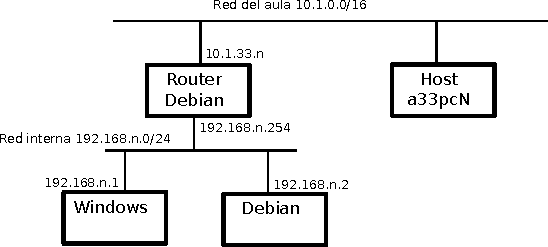
\includegraphics[width=0.5\textwidth]{media/practica-red-ip.pdf}
\caption{\label{fig:conexiones-de-red-alumno}Diagrama de conexiones de red}
\end{figure}

La conectividad IP puede comprobarse con comandos como \texttt{ping}, \texttt{pathping}, \texttt{mtr} o \texttt{tracert}


\section{Características de las máquinas virtuales}
\label{sec:org0000006}
\begin{itemize}
\item El \emph{router} Debian deberá ser configurado sin utilizar el modo gráfico ni \emph{network manager}
\item Se recomienda utilizar distribuciones Debian frente a Ubuntu, por el ahorro de memoria RAM. Sin entorno gráfico, Debian funciona correctamente con 512MB.
\item Por la misma razón, Windows 7 es preferible a Windows 10 o Windows 11.
\item El número \emph{n} corresponde con el número de identificación del PC real en clase, que se apuntará en esta hoja de cálculo: \href{http://bit.ly/2sji9gQ}{http://bit.ly/2sji9gQ}
\end{itemize}


\section{Enrutamiento}
\label{sec:org0000009}
Conecta tus máquinas virtuales a las del resto del aula como se indica en la figura \ref{fig:conexiones-de-red-aula}.
\begin{itemize}
\item Activa el enrutamiento en el \emph{router} Debian
\item Configura las tablas del \emph{router} Debian para que enrute hacia el resto de redes de tus compañeros
\item Comprueba que:
\begin{enumerate}
\item Tu \emph{router} Debian contacta con el resto de \emph{routers} Debian
\item Tu \emph{router} Debian contacta con el resto de máquinas reales
\item Tus ordenadores \emph{hosts} (Windows y Debian) pueden contactar con otros \emph{routers} Debian
\item Tus ordenadores \emph{hosts} pueden contactar con otros ordenadores \emph{hosts}
\end{enumerate}
\item \textbf{Nota}: la comunicación entre las máquinas reales y los ordenadores \emph{hosts} queda fuera de esta práctica
\end{itemize}

\begin{figure}[htbp]
\centering
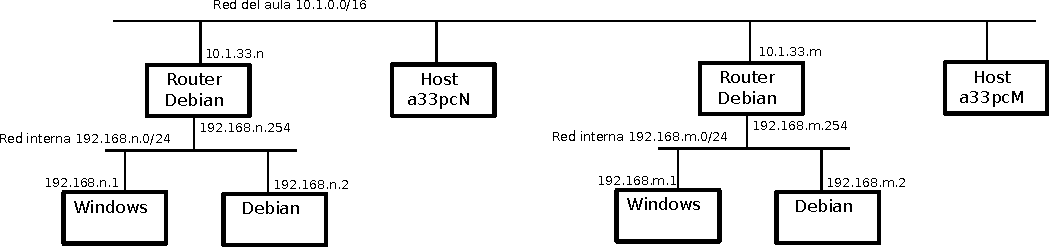
\includegraphics[width=.9\linewidth]{media/practica-enrutamiento-ip.pdf}
\caption{\label{fig:conexiones-de-red-aula}Diagrama de conexiones de red en el aula}
\end{figure}

La conectividad IP puede comprobarse con comandos como \texttt{pathping}, \texttt{mtr} o \texttt{tracert}. \texttt{ping} no es válido, pues no muestra los saltos del enrutamiento.

\section{Reinicio}
\label{sec:org000000c}
La configuración realizada en el \emph{router} puede que no sea persistente, y no se mantiene tras un reinicio. Investiga cómo puede conseguirse que al reiniciar siga funcionando el enrutamiento.

\section{Qué se valorará}
\label{sec:org000000f}
Se entregará un documento (entrada de blog, \texttt{DOCX}, \texttt{PDF} \ldots) con los pasos que se han seguido para la creación de la red y su configuración, así como la salida de los comandos que muestran la conectividad de los ordenadores.

Se tendrá en cuenta:
\begin{itemize}
\item La corrección técnica
\item Que siga funcionando tras un reinicio
\item La claridad
\begin{itemize}
\item Diagramas, pruebas de funcionamiento, instrucciones completas \ldots
\end{itemize}
\item La apariencia profesional
\begin{itemize}
\item Presentación, gramática, ortografía, homogeneidad \ldots
\end{itemize}
\end{itemize}



\section{Instrucciones de entrega}
\label{sec:org0000012}
\begin{itemize}
\item El ejercicio se realizará y entregará de manera
individual.
\begin{itemize}
\item Solo se admiten trabajos en pareja, si en clase es necesario compartir ordenador.
\end{itemize}
\item Sube el documento a \href{https://aulavirtual3.educa.madrid.org/ies.alonsodeavellan.alcala/course/view.php?id=189}{la tarea correspondiente en el aula virtual}
\item Presta atención al plazo de entrega (con fecha y hora).
\end{itemize}
\end{document}